\chapter[SM-ID of block structured nonlinear systems]{Set-membership identification of block structured nonlinear systems}

\section{Introduction}
Let us continue to generalize our Set-Membership identification framework introducing the theoretical concepts useful to identify \textbf{SISO nonlinear systems} in the regression form we have seen in the very first part of these notes:

\begin{figure}[h]
   \centering
   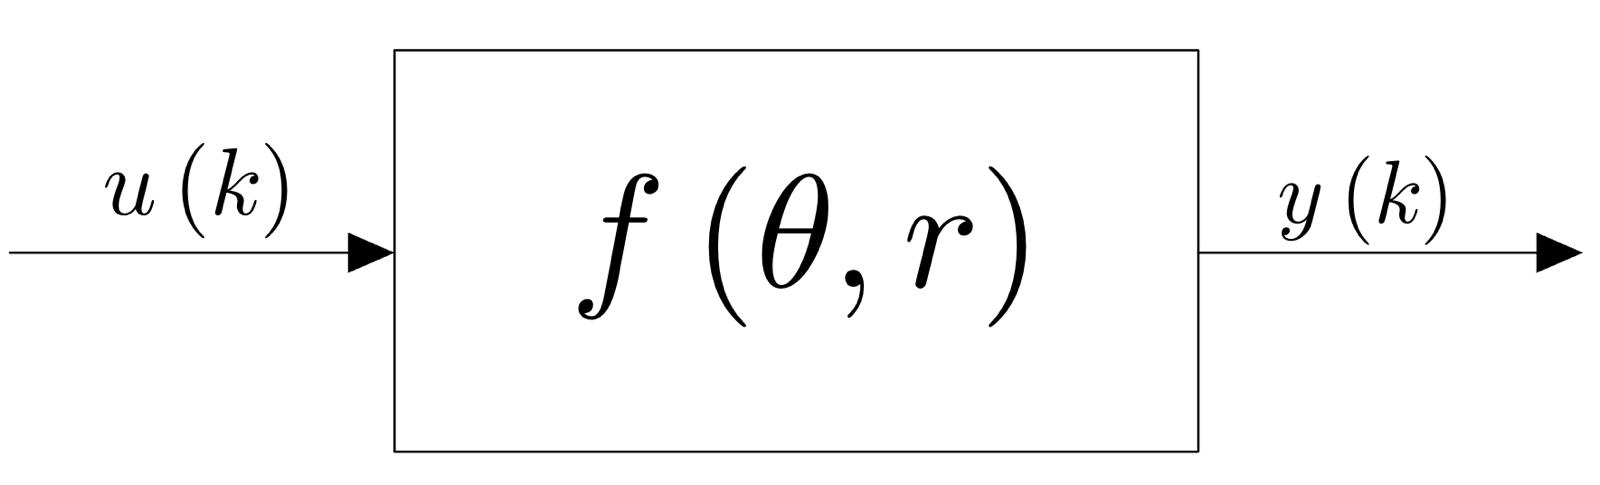
\includegraphics[scale=0.15]{img/nonlinear.jpeg} 
   \caption{Nonlinear SISO system (regression form)}
\end{figure}
\vspace{-1cm}
\begin{equation}
    y(k)=f(\theta,r(k))=f(\theta, [y(k-1),y(k-2),\dots,y(k-n), u(k), u(k-1), \dots, u(k-m)])
\end{equation}
where $\theta$ is the vector with the parameters of the model, while $r(k)$ is the so-called \textbf{regressor}. We specialize the class $f$ of functions we deal with, in particular they are \textbf{multivariate polynomial function of the regressor $r(k)$}. In this context we propose some examples which, as usual, are useful to both introduce and better clarify the setting to which we are approaching. Through all of the examples we do two fundamental quantities are:
\begin{itemize}
    \item The \textbf{dynamical order of the system} $n$; this is related to the number of past samples we need in order to describe the generic system output $y(k)$; 
    \item The \textbf{degree} (or \textbf{order}) $\deg(f)$ of the multivariate polynomial $f$ describing the nonlinear system in the parametrized form.
\end{itemize}

\subsubsection{Example 1}
Suppose that from the physical insights we know that the system has $n=1$ and $\deg(f)=2$. This is the same to state that the equation describing the I/O of the system is:
\begin{align}
    y(k)&=f(\theta,r(k))=f(\theta,[y(k-1),u(k),u(k-1)])=\\
    &=\theta_1y(k-1)+\theta_2 u(k) + \theta_3 u(k-1) 
    + \theta_4 y^2(k-1)+\theta_5 u^2(k)+\theta_6 u^2(k-1)+\\
    &+\theta_7{y(k-1)u(k)}+\theta_8{y(k-1)u(k-1)}+\theta_9{u(k)u(k-1)}
\end{align}

Since $\deg(f)=2$, in order to avoid loosing of generality we have to consider also the mixed monomial terms of order 2.

\subsubsection{Example 2}
Let us consider, now, the case in which both the dynamical order and multivariate polynomial degree are the same as before, on the other hand from the physical insights we know that the structure of the I/O equation is:
\begin{equation*}
    y(k)=\theta_1y(k-1) + \theta_2 u(k) +\theta_3 u^2(k-1)+\theta_4{y(k-1)u(k)}
\end{equation*}
It is not said that all of the terms are present, in this case there is some reason for which this happens.

\subsubsection{Example 3}
Finally, here we consider the case in which, again, $n$, $\deg(f)$ are equal while not having any useful physical insights which can allow us make a guess on the shape of $f(\theta,r)$.
In this particular case some general assumptions on the continuity\footnote{
    for example $f\in\mathcal{C}^0$ or $f\in\mathcal{C}^1$
} of $f$ are needed, otherwise we cannot say anything and the identification problem is not tractable. This example gives the possibility to introduce to cite an important result.

\section{Dealing with nonlinearity of the problem}
Whether one can assume that the function $f$ can leverage on some continuity properties,the \textbf{Stone-Weirstrass theorem} can be used. It allows us with the possibility to approximate as well as we want the true nonlinear function with a multivariate polynomial over a \textit{compact set}. In spite this is a nice result, it is not going to provide a way to build such polynomial, since it is an \textit{existency theorem}.

\subsection{On the choice of the polynomial structure}
When we are not provided with physical insights making us to neglect some terms of the multivariate polynomial, we can always start from a \textit{complete description}, next when the identification procedure is performed, the terms which are not included into the model description will have an uncertainty interval whose central estimate is approximatively equal to zero.

Having said that, the choice of $\deg(f)$ can be done by using the following \textbf{procedure}: 
\begin{enumerate}
    \item[0.] We can start from $\deg(f)=2$\footnote{
        If there was $\deg(f)=1$ the system under study is linear
    } and we try to solve the problem going through the computation of the feasible parameter set $\mathcal{D}_\theta$ putting together all the available information;\item[1.]\textbf{\large Is the $\mathcal{D}_\theta$ empty?}\footnote{
        Practically speaking, using \texttt{SparsePOP} a symptom of the fact that $\mathcal{D}_\theta=\varnothing \ \iff $ POP infeasible can be read in the output variable \texttt{exitflag}, in particuar its negativeness implies the infeasibility of the POP. 
    }
    \begin{itemize}
        \itemsep-0.3em
        \item {\Large{\color{green}\underline{\textbf{NO}}}} In this case we have to check what are the (relaxed) PUI, in particular we have to check that
        \begin{equation} \label{eq:extrema_sign}
            \text{sign}(\underline{\theta}_i) = 
            \text{sign}(\overline{\theta}_i) \quad i=1,\dots,n_\theta
        \end{equation} 
        Whether this is the case we can accept our solution and use the retrieved interval in order to simulate control the identified system. On the other hand, we continue to investigate in the fact that, maybe the the length of the PUI
        \begin{equation}
            \vert \underline{\theta}_i-\overline{\theta}_i \vert \le \delta
        \end{equation}
         for some small $\delta$. In pratice this is the case when, if for the other parameters the property (\ref{eq:extrema_sign}) is fulfilled, the procedure is saying us that $\theta_i=0$. On the contrary if (\ref{eq:extrema_sign}) is not satisfied and the noise bound is big\footnote{
            We can quantify it in percentage terms with respect to the measured input $\tilde{u}(k)$ or output $\tilde{y}(k)$.
         }, it would be better if the sensor is changed because it is not properly measuring the data to be used in the identification process. Finally on the other side when the \textit{sign concordance property} is not fulfilled and the noise relative bound is acceptable, \textbf{the order of the polynomial ought to be increased} $\to$ try $\deg(f)=\deg(f)+1$. 
     \end{itemize} 
    \item {\Large{\color{red}\underline{\textbf{YES}}}} Also in this case the $\deg(f)$ is too \textbf{low}, then you have to increase it.
\end{enumerate}

\noindent
\begin{remark}[\textbf{Unknown dynamical order} $n$]
    A similar \textit{trial and error} approach can also be applied to the case (both linear and nonlinear systems) when the \textit{dynamical order $n$} is not exactly known from the physical insights. This will be useful especially when the Direct Data-driven control technique will be explained.
\end{remark}

\noindent
\subsection{Additional comments on the PUIs extrema sign concordance}
After this discussion, let us give further attention on the property (\ref{eq:extrema_sign}). The reason why we must reject the PUIs with non-concordant sign is that we cannot even know the sign for a certain parameter. Whether we want to design a simple stabilizing \textit{feedback controller}, the fact that we do not have the information on the sign does not protect us from building a positive feedback(!), making unstable the closed loop system. We conclude this part saying that the \textbf{relative size of the uncertainty} is given by: 
\begin{equation}
    \Delta_i = \bigg\vert \frac{\overline{\theta}_i-\underline{\theta}_i}{\theta_i^c} \bigg\vert, \qquad
    \theta_i^c = \frac{\overline{\theta}_i+\underline{\theta}_i}{2}
\end{equation}
where $\theta_i^c$ is the so-called \textbf{central estimate}  which can leverage on some nice properties how we will see in one of the next chapters. When the sign of the extrema is not the same, the uncertainty relative size is greater than the 1 (that is 100\%).

\section{Toward the computational load reduction}
We have seen in the previous sections a trial and error procedure for choosing either the dynamical order or the order of the multivariate polynomial $f$. The drawback of such an approach is that the computational complexity explode when the such a polynomial have high order. Practical examples are the best way to understand things. Let us do, then, an example.

\subsubsection{Example}
Suppose we want to estimate the parameters of the following nonlinear MISO system:
\begin{equation*}
    y(k)=\theta_1{u_1(k)}+\theta_2{u_1(k)u_2(k)}+\dots+
    +\theta_p{u_1(k)\dots{u_p(k)}}
\end{equation*}
If we add the fact that both the inputs and the output are corrupted by bounded measurement noise. The feasible parameter set is defined as:
\begin{equation}
    \begin{aligned}
        \mathcal{D}_\theta = \{
        \theta\in\mathbb{R}^p: \ &\tilde{y}(k)-\eta(k) = \theta_1 (\tilde{u}(k)-\xi_1(k)) + \theta_2 (\tilde{u}_1(k)-\xi_1(k)) (\tilde{u}(k)-\xi_2(k)) +\dots\\
        &\theta_p (\tilde{u}_1(k)-\xi_1(k))\dots(\tilde{u}_p(k)-\xi_p(k)) \quad k=n+1,...,N\\
        &\vert \eta(k) \vert \le \Delta_\eta \ k=1,...,N\\
        &\vert \xi_i(k) \vert \le \Delta_xi \ k=1,...,N \ i=1,...,p
    \}
    \end{aligned}
\end{equation}
Now, considering the problem of computing the PUIs, we have to solve a POP whose constraints are at most of order $p+1$. Moreover, if $p$ is high, the minimum order of relaxation $\delta_{min}$ is high. Bad symptom! In order to \textbf{reduce the computational complexity} of the POP we can reformulate it by introducing new variables $z_j$ as follows:

\begin{equation*}
    \begin{aligned}
        &\min_{\theta,\xi,\eta,z}  \theta_1\\
        &\text{s.t.} \quad z_1(k)=\xi_1(k)\cdot\xi_2(k), \ 
        z_2(k)=z_1(k)\cdot\xi_3(k), \ \dots, \ z_{p-1}(k)=z_{p-2}(k)\cdot{\xi_p}(k)\\
        &\tilde{y}(k)-\eta(k)=\theta_1{u_1(k)}+\theta_1{\xi_1(k)}+\theta_2+\dots+\theta_p{z_{p-1}}
    \end{aligned}
\end{equation*}
All of the constraints entering the optimization problem are now bilinear, then we can pick as minimum order of relaxation $\delta_{\min}=1$.

\section{Block-oriented nonlinear systems}
The SysId procedure for nonlinear system is quite challenging. When we have addressed the problem of identifying an LTI system (both SISO and MIMO), we had the information about the transfer function that was of crucial importance. For nonlinear system we cannot exploit such an information. In the most general case, assuming we can do some continuity assumptions, we can go through the steps we have described in order to identify the system, otherwise we have to exploit as much as possible the \textit{a-priori information} available on that system. In many situations we can know something about the \textbf{internal structure of the nonlinear system}. To this aim we propose the so-called \textbf{block-structured nonlinear systems}.

\begin{definition}[Block oriented nonlinear systems] Block oriented nonlinear systems are nonlinear dynamical systems which are obtained by \textbf{connecting together} a number of subsystems such that each one of the subsystems can either be:
\begin{itemize}
    \itemsep-0.3em
    \item a \textit{dynamical LTI system}
    \item a \textit{static nonlinear system}
\end{itemize}

\subsection{Hammerstein system}

This structure is characterized by the following features:
\begin{enumerate}
    \itemsep-0.3em
    \item Internal signal $x(k)$ cannot be measured;
    \item It is useful to describe physical systems which are essentially LTI systems but with a \textbf{significant input nonlinearity} such as input saturation, dead-zone and any other non linear effect in the actuation part.
\end{enumerate}
\begin{figure}[h]
    \centering
    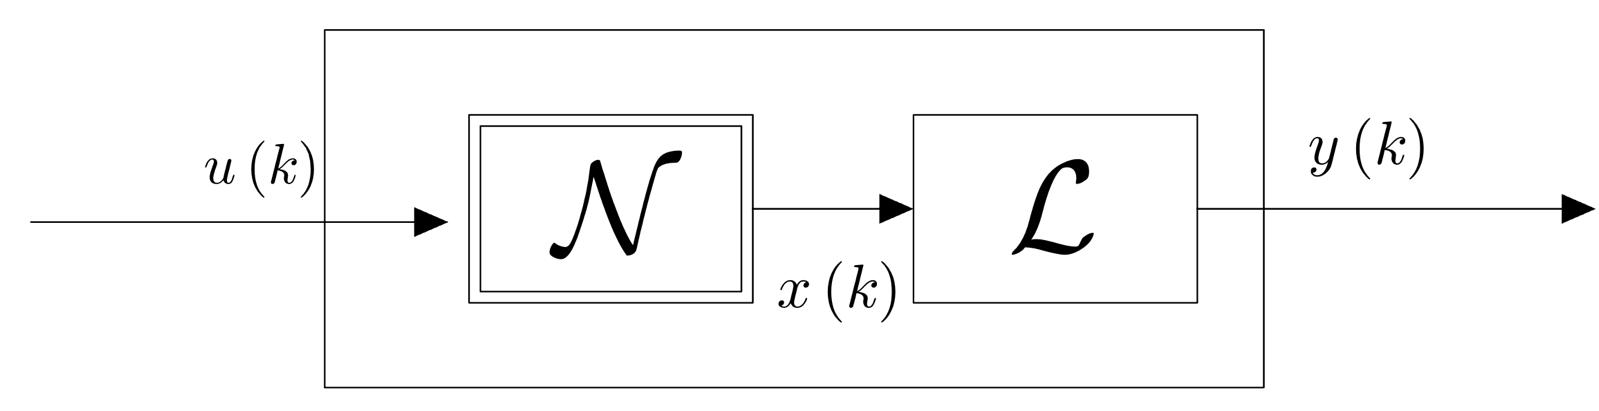
\includegraphics[scale=0.15]{img/hammer.jpeg}
    \caption{Hammerstein system (block diagram)}
\end{figure}
The nonlinear part is often referred as $\mathcal{N}(\cdot)$ and it is a function of $u(k)$, while the linear part $\mathcal{L}$ is represented by a transfer function $G(q^{-1})$.
    
\end{definition}

